\section{RNN}
    RNN的总体结构如图\ref{fig:rnnarchitecture}所示。

    \begin{figure}[H]
        \centering
        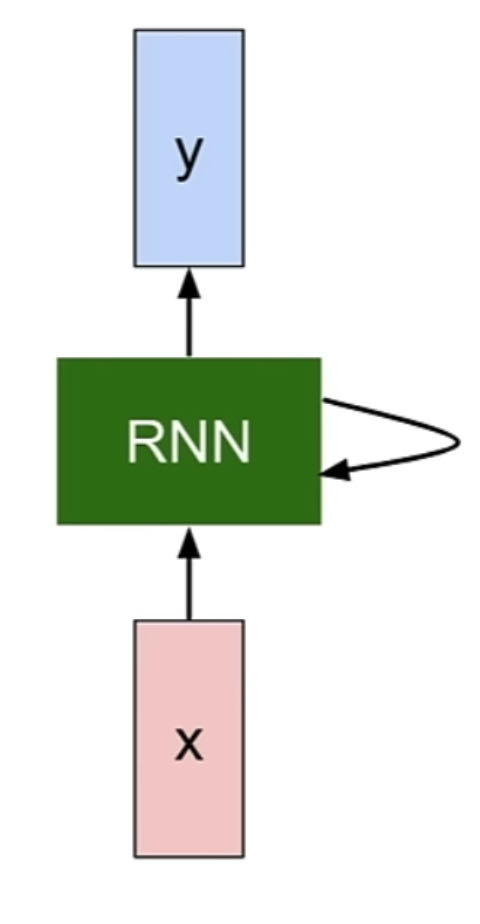
\includegraphics[width=0.07\textheight]{./figures/rnnarchitecture.jpg}
        \caption{RNN结构}
        \label{fig:rnnarchitecture}
    \end{figure}

    在$t$时刻,通常用$h_t$代表隐藏层的状态,$x_t$代表输入,$y_t$代表输出。
    于是隐藏层的状态更新可以用

    \begin{equation}
        h_t = f_W (h_{t-1}, x_t)
    \end{equation}
    来表达。一个比较简单的例子为双曲正切函数,即$h_t = \tanh (W_{hh} h_{t-1} + W_{xh} x_t)$。

    对于不同的场景,RNN的计算图有不同的形式。
    例如,生成图像标题的RNN计算图为单一输入到多输出,
    机器翻译的RNN计算图为多输入到多输出。
    本次实验采用的RNN结构为单一输入到单一输出,
    利用每一个时间步的输入来预测下一个时间步的输出。
    原始输入节选自China Daily在2024年7月25日发布的
    World hails success of historic Palestinian unity declaration
    和
    Expert: Pursuit of new tech should be sensible,
    利用One-Hot编码处理后训练RNN模型,得到的损失曲线如图\ref{fig:RNNlosshistory}所示,
    权重矩阵热力图如图\ref{fig:rnnweightmatrix}所示。

    \begin{figure}[H]
        \centering
        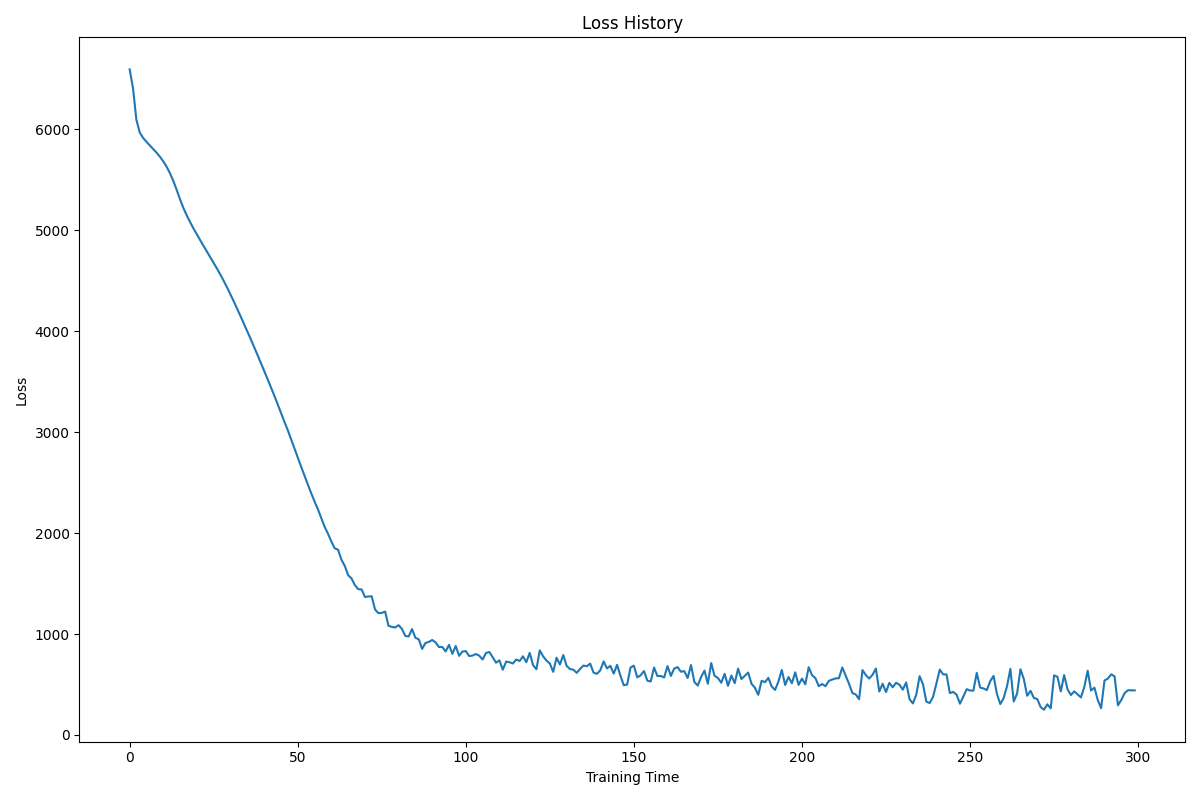
\includegraphics[width=0.7\linewidth]{../output/rnn/no scheduler/rnnloss.png}
        \caption{RNN损失曲线}
        \label{fig:RNNlosshistory}
    \end{figure}

    \begin{figure}[H]
        \centering
        \begin{subfigure}{0.3\textwidth}
            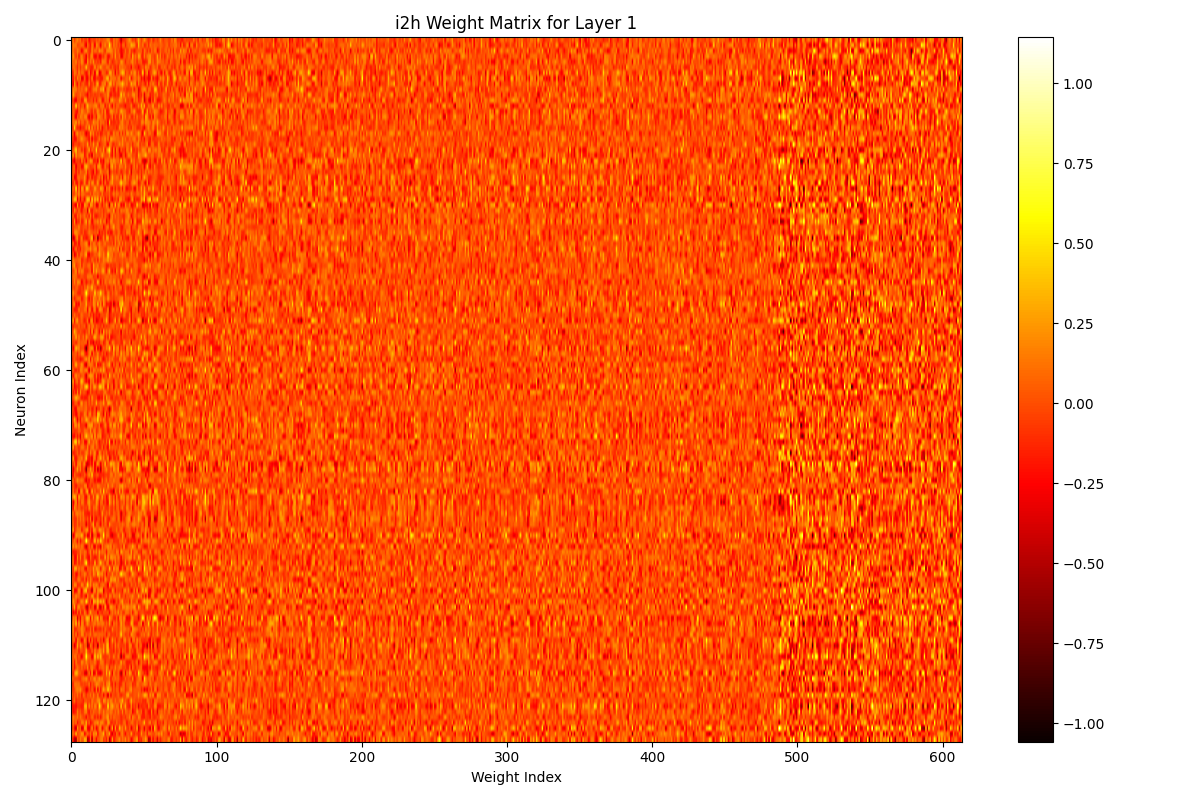
\includegraphics[width=\linewidth]{../output/rnn/no scheduler/Weight Matrix for Layer 1.png}
            \caption{第1层}
            \label{fig:rnnweightmatrixforlayer1}
        \end{subfigure}
        \hfill
        \begin{subfigure}{0.3\textwidth}
            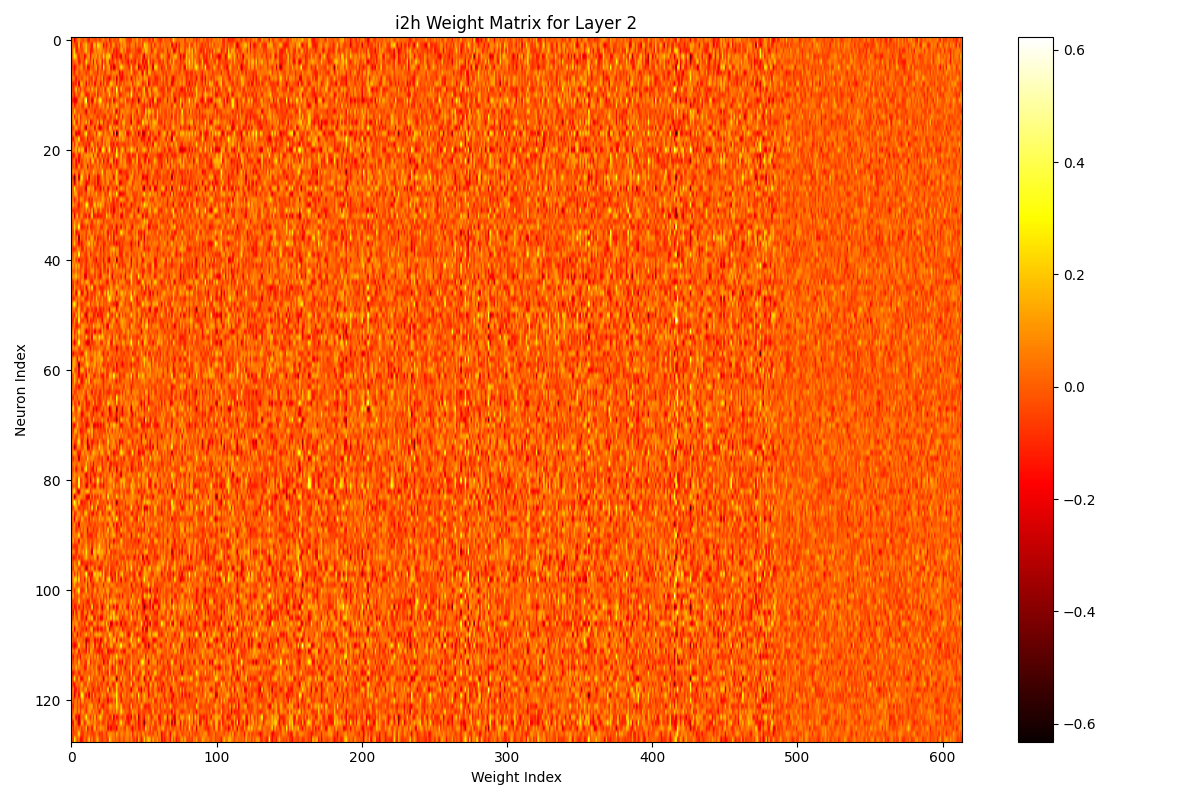
\includegraphics[width=\linewidth]{../output/rnn/no scheduler/Weight Matrix for Layer 2.png}
            \caption{第2层}
            \label{fig:rnnweightmatrixforlayer2}
        \end{subfigure}
        \hfill
        \begin{subfigure}{0.3\textwidth}
            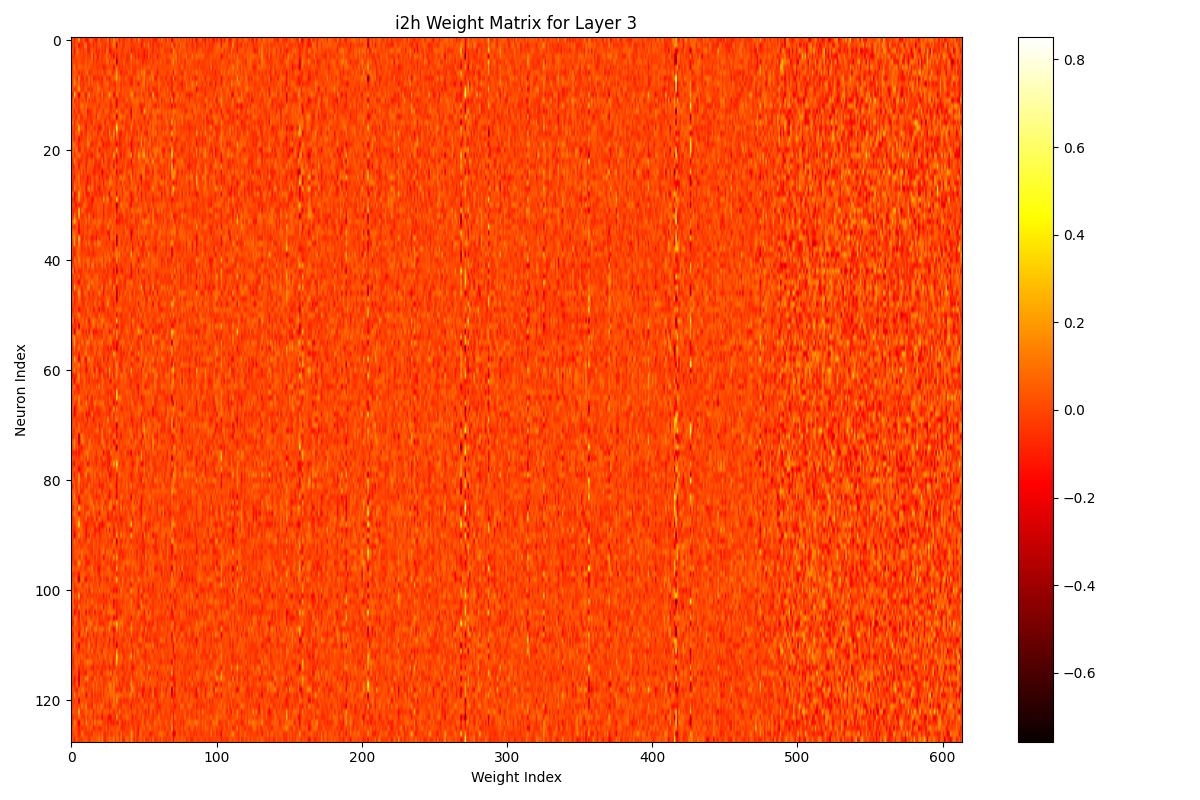
\includegraphics[width=\linewidth]{../output/rnn/no scheduler/Weight Matrix for Layer 3.png}
            \caption{第3层}
            \label{fig:rnnweightmatrixforlayer3}
        \end{subfigure}
        \caption{RNN隐藏层权重矩阵}
        \label{fig:rnnweightmatrix}
    \end{figure}

    注意到损失值在经历多轮训练之后并未完全收敛,损失曲线存在较多的毛刺,模型出现了局部退化的现象。
    此处可以采用学习率调度机制来改善训练过程,
    在模型的训练过程中添加ReduceLROnPlateau调度器,
    factor设置为0.1,mode设置为min,patience设置为5,
    处理后得到的损失曲线如图\ref{fig:RNNlosshistorywithscheduler}所示,
    权重矩阵热力图如图\ref{fig:rnnweightmatrixwithscheduler}所示。

    \begin{figure}[H]
        \centering
        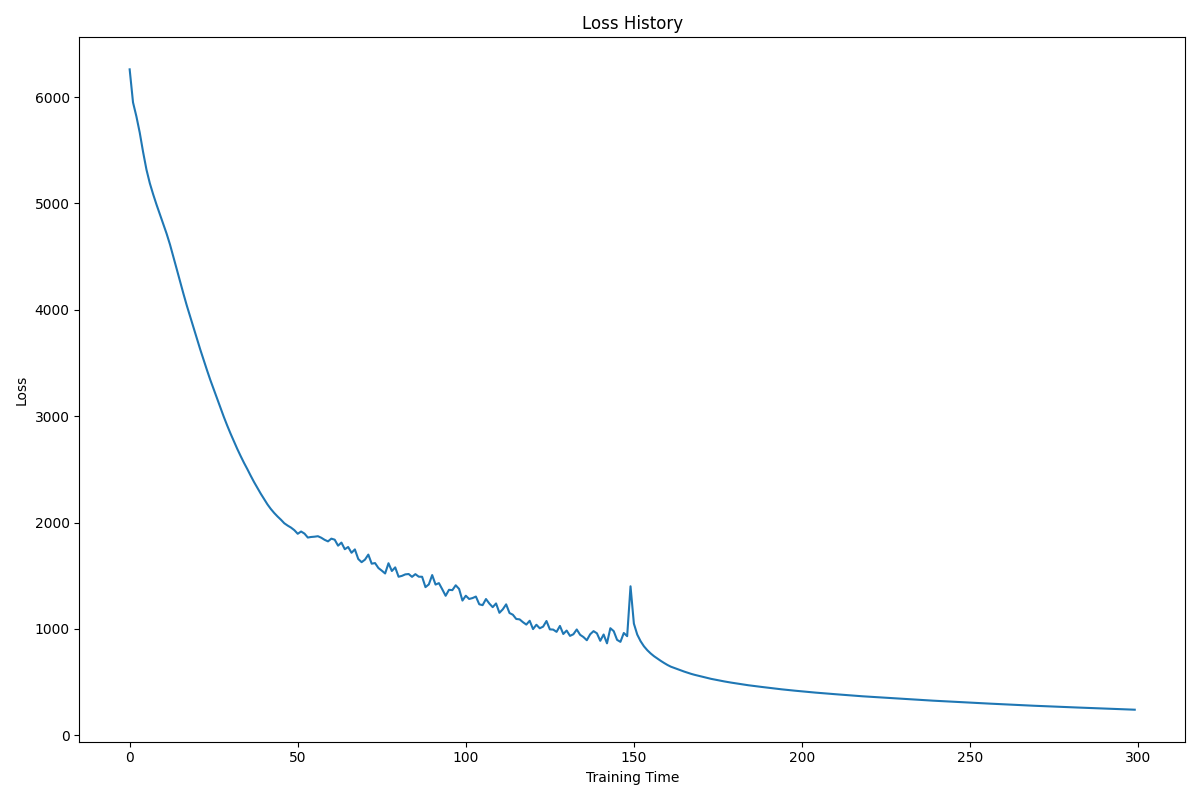
\includegraphics[width=\linewidth]{../output/rnn/with scheduler/rnnloss.png}
        \caption{RNN损失曲线}
        \label{fig:RNNlosshistorywithscheduler}
    \end{figure}

    \begin{figure}[H]
        \centering
        \begin{subfigure}{0.3\textwidth}
            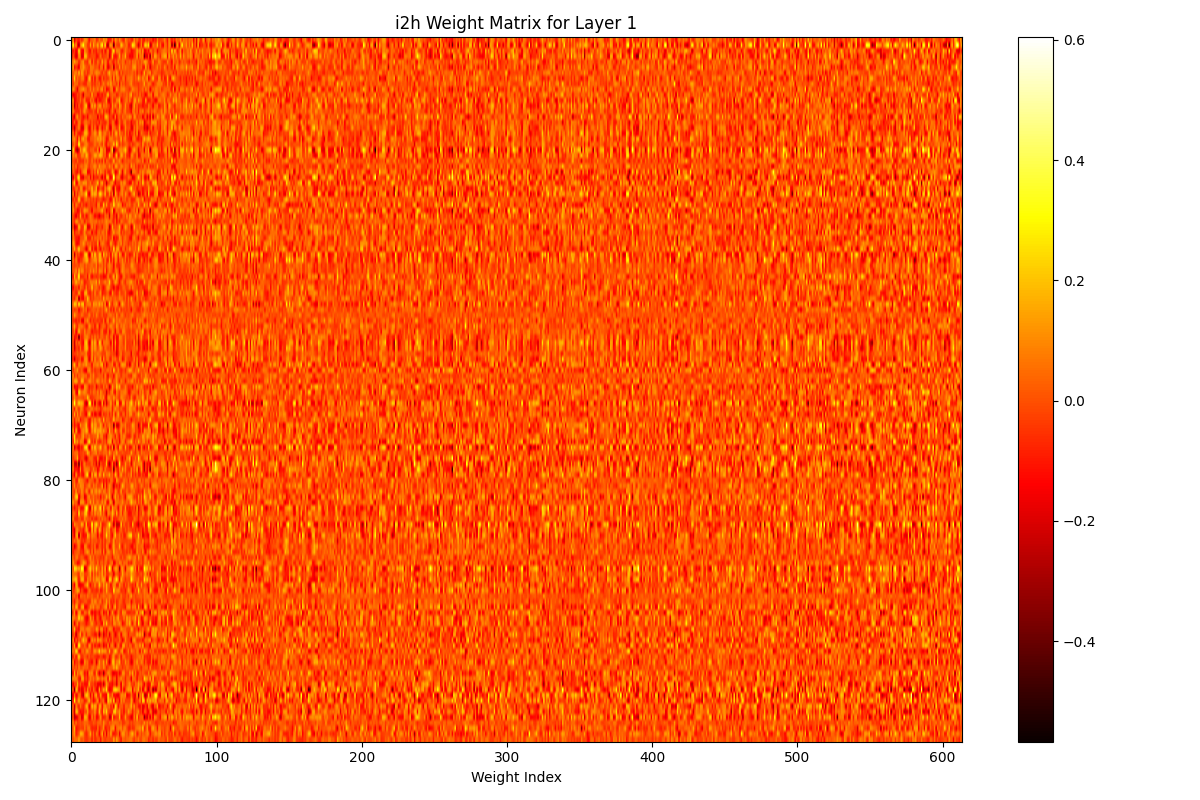
\includegraphics[width=\linewidth]{../output/rnn/with scheduler/Weight Matrix for Layer 1.png}
            \caption{第1层}
            \label{fig:rnnweightmatrixforlayer1withscheduler}
        \end{subfigure}
        \hfill
        \begin{subfigure}{0.3\textwidth}
            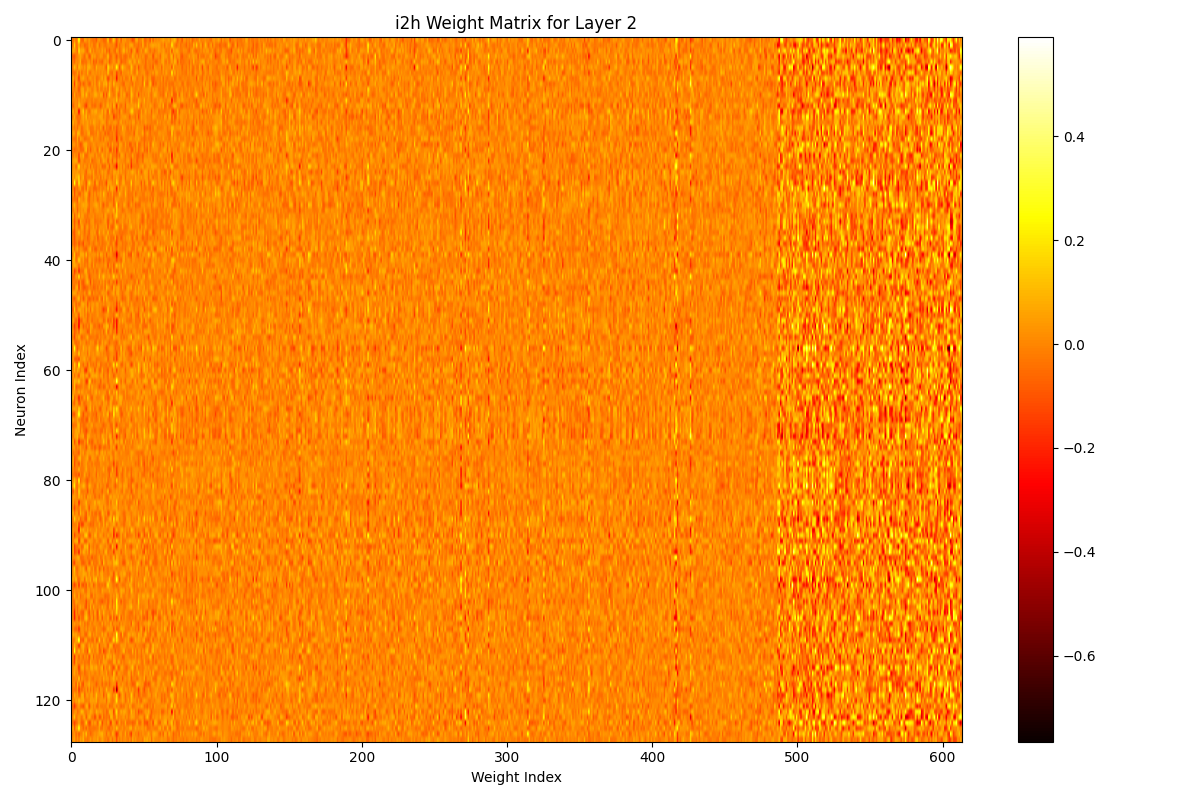
\includegraphics[width=\linewidth]{../output/rnn/with scheduler/Weight Matrix for Layer 2.png}
            \caption{第2层}
            \label{fig:rnnweightmatrixforlayer2withscheduler}
        \end{subfigure}
        \hfill
        \begin{subfigure}{0.3\textwidth}
            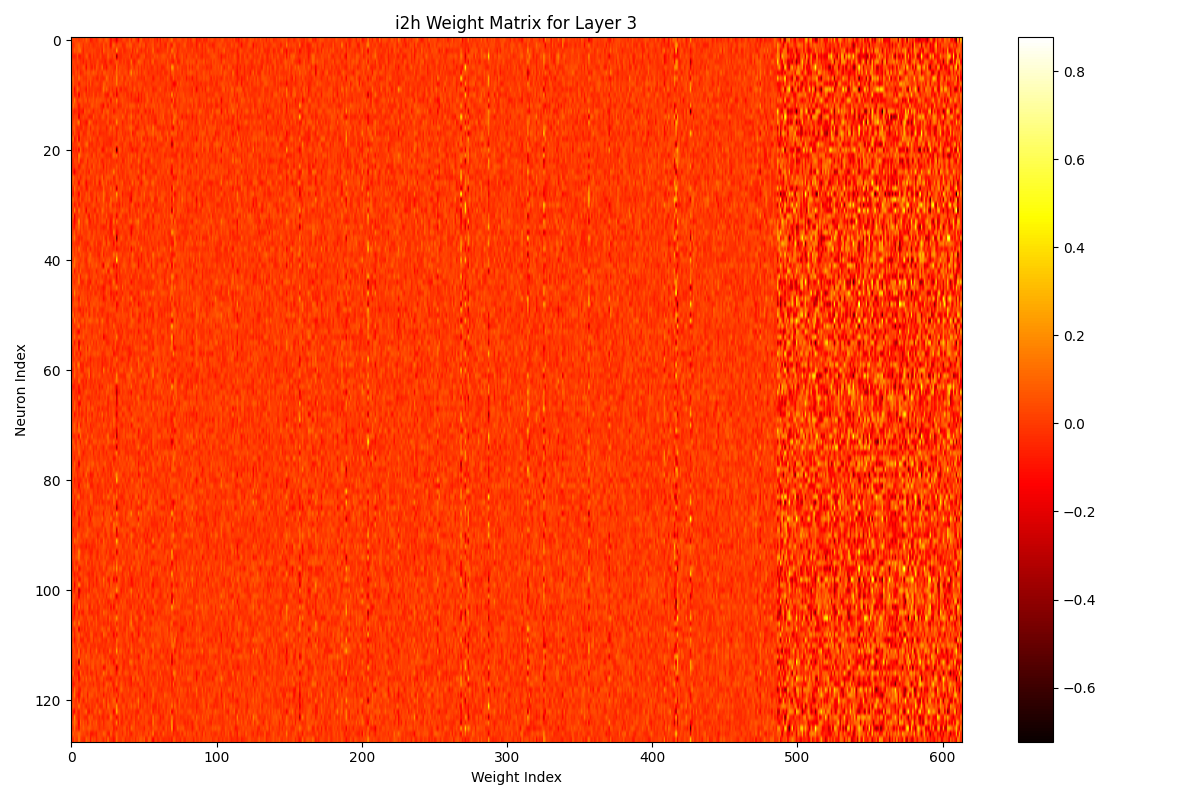
\includegraphics[width=\linewidth]{../output/rnn/with scheduler/Weight Matrix for Layer 3.png}
            \caption{第3层}
            \label{fig:rnnweightmatrixforlayer3withscheduler}
        \end{subfigure}
        \caption{RNN隐藏层权重矩阵}
        \label{fig:rnnweightmatrixwithscheduler}
    \end{figure}

    分别调用两次训练后的RNN模型,输入提示词china后,设置生成文本长度为100,得到的结果如图\ref{fig:rnntext-comparison}所示。

    \begin{figure}[H]
        \centering
        \begin{subfigure}[b]{0.45\textwidth}
            \textit{"china for facilitating talks among hamas fatah and 12 other palestinian factions anwar said that have different competitive advantages to play to china's people to leverage the formation of new production factor lin further said china needs to reform its financial system to better mobilize financial resources for supporting innovations while implementing fiscal reforms to better balance spending responsibilities between local and central governments encouraging the development of venture capital and patient capital will be important improvements he said li dongsheng founder and chairman of chinese consumer electronics maker tcl technology group corp said china's new growth drivers come from industrial"}
            \caption{不使用调度器}
            \label{fig:rnntextnoscheduler}
        \end{subfigure}
        \hfill
        \begin{subfigure}[b]{0.45\textwidth}
            \textit{"china must stand in solidarity with the palestinian people and urge israel to end its brazen violence which has destroyed gaza and killed around 40000 innocent palestinians in the past 10 months sharif said pakistan reaffirms its unwavering support for the palestinian cause and reiterates its call for a two-state solution that creates an independent state of palestine with pre-1967 borders he added the foreign ministry of turkiye welcomed in a statement the gathering of palestinian factions has been broadly hailed as an exceptional success in china's diplomatic efforts to create conditions for lasting peace in gaza and urged nations that"}
            \caption{使用调度器}
            \label{fig:rnntextwithscheduler}
        \end{subfigure}
        \caption{RNN生成文本比较}
        \label{fig:rnntext-comparison}
    \end{figure}